% !TEX TS-program = XeLaTeX
% !TEX spellcheck = en-US
\documentclass[aspectratio=169]{beamer}

\usetheme{example}

\title{Lecture 3:\\ LDA and regularized regression analysis}
\institute{GRA4160: Predictive modelling with machine learning}
\date{January 23rd 2025}
\author{Vegard H\o ghaug Larsen}

\begin{document}

\maketitle

\frame{
	\frametitle{Progress on mini project}

	\begin{itemize}
		\item Presentation: March 20th
		\item I've added an excel sheet to Itslearning. Please fill in your group members and the topic you want to work on.
		\pause
		\bigskip
		\item[] \underline{\bf Some possible topics}:
		\smallskip
		\item \textbf{Image Classification}: Train a model or models to classify images into different categories, such as animals, objects, etc. using a public dataset like: \href{https://www.cs.toronto.edu/~kriz/cifar.html}{CIFAR} or \href{http://yann.lecun.com/exdb/mnist/}{MNIST}.
		\item \textbf{Sentiment Analysis}: Train a classifier to predict the sentiment (positive, negative, neutral) of a piece of text (e.g., movie reviews, product reviews, etc.) using a public dataset like \href{https://ai.stanford.edu/~amaas/data/sentiment/}{Large Movie Review Dataset} or \href{https://www.yelp.com/dataset}{Yelp} reviews.
		\item \textbf{Macroeconomic forecasting}: Predict macro variables with ML methods such as random forest or neural nets. One possible dataset is \href{https://research.stlouisfed.org/econ/mccracken/fred-databases/}{FRED-MD}.
	\end{itemize}
}

\frame{
	\frametitle{Plan for today:}

	\begin{enumerate}
		\item Recap from last week: Supervised learning
		\item Linear discriminant analysis
		\item Regularized regression analysis
		\item Exercise: Predicting house prices
	\end{enumerate}
}

\begin{frame}
    \frametitle{Recap: Machine Learning Basics}
    \begin{itemize}
        \item \textbf{Machine Learning} enables computers to learn patterns from data.
        \item Three main paradigms:
            \begin{itemize}
                \item \textbf{Supervised} learning (labeled data).
                \item \textbf{Unsupervised} learning (unlabeled data).
                \item \textbf{Reinforcement} learning (reward-based).
            \end{itemize}
        \item \textbf{Bias-Variance Trade-off}: Balancing underfitting (\textit{high bias}) vs. overfitting (\textit{high variance}).
        \item Ultimate goal: \textbf{Generalize well} to new, unseen data.
    \end{itemize}
\end{frame}

\begin{frame}
    \frametitle{Recap: Supervised Learning models}
    \begin{itemize}
        \item \textbf{Linear Regression}
            \begin{itemize}
                \item Predicts continuous outcomes.
                \item Parametric model minimizing MSE.
                \item Useful for both prediction \& inference.
            \end{itemize}
        \item \textbf{k-Nearest Neighbors (kNN)}
            \begin{itemize}
                \item Non-parametric, instance-based.
                \item Classification/regression by majority vote/mean of nearest neighbors.
                \item Choosing $k$ is crucial to avoid over/underfitting.
            \end{itemize}
        \item \textbf{Naive Bayes}
            \begin{itemize}
                \item Relies on Bayes' Theorem with a ``naive'' independence assumption.
                \item Often used for text classification (e.g., spam detection).
                \item Simple, fast, surprisingly effective despite strong assumptions.
            \end{itemize}
    \end{itemize}
\end{frame}


%\frame{
%	\frametitle{Linear discriminant analysis}
%	\begin{itemize}
%		\item Linear discriminant analysis (LDA) is a classification method
%		\item LDA finds a linear combination of the features that maximizes the separation between classes
%		\item Assumptions for LDA:
%		\begin{enumerate}
%			\item The classes are normally distributed
%			\item The classes have the same covariance matrix
%			\item The classes are linearly separable
%		\end{enumerate}
%		\item We will look at how this can be implemented in Scikit-learn
%	\end{itemize}
%}

\frame{
    \frametitle{Introduction to Linear Discriminant Analysis (LDA)}
    \begin{itemize}
        \item \textbf{Definition:} LDA is both a \emph{classification} and \emph{dimensionality reduction} technique.
        \item \textbf{Core idea:} Project data onto a lower-dimensional space (often 1D) that maximizes class separability.
        \pause
        \item \textbf{Typical Uses:}
        \begin{itemize}
            \item Face recognition
            \item Medical diagnosis
            \item Market research
        \end{itemize}
        \pause
        \item \textbf{Why LDA?} 
        \begin{itemize}
            \item Simple, interpretable linear boundaries.
            \item Often effective when class distributions are approximately Gaussian.
            \item Can reduce noise by focusing on most discriminative directions.
        \end{itemize}
    \end{itemize}
}

\frame{
    \frametitle{When to Use LDA}
    \begin{itemize}
        \item \textbf{Two or more classes:} LDA can handle multi-class classification by finding multiple discriminant components.
        \item \textbf{Data separability:} Works well when classes are well-separated and covariance is similar across classes.
        \item \textbf{Dimensionality reduction:} When you need a lower-dimensional representation for further analysis or visualization.
        \pause
        \item \textbf{Comparison to Other Methods:}
        \begin{itemize}
            \item \textbf{Logistic Regression:} Also linear, but does not reduce dimensionality.
            \item \textbf{Quadratic Discriminant Analysis (QDA):} Allows different covariance matrices per class, but is more complex.
            \item \textbf{Nearest Neighbors:} Non-parametric, can be less interpretable in high dimensions.
            \item \textbf{Principal Component Analysis (PCA):} Unsupervised, focuses on variance rather than class separation.
        \end{itemize}
    \end{itemize}
}

\frame{
    \frametitle{Mathematical Foundations of LDA}
    \begin{itemize}
        \item \textbf{Objective:} Maximize between-class variance while minimizing within-class variance.
        \item \textbf{Scatter Matrices:}
        \begin{itemize}
            \item \(\mathbf{S}_B\) (Between-class scatter) captures how class means differ.
            \item \(\mathbf{S}_W\) (Within-class scatter) captures how data points vary around their class means.
        \end{itemize}
        \item \textbf{Optimization:}
        \[
            \mathbf{w} = \arg \max_{\mathbf{w}} \; \frac{\mathbf{w}^T \mathbf{S}_B \, \mathbf{w}}
            {\mathbf{w}^T \mathbf{S}_W \, \mathbf{w}}.
        \]
        \item The vector \(\mathbf{w}\) defines the projection that best separates the classes in a low-dimensional subspace.
    \end{itemize}
}

\frame{
    \frametitle{Deeper Dive: How \(\mathbf{w}\) is Computed}
    \begin{itemize}
        \item \textbf{Class Means:} 
        Let \(\mathbf{m}_i\) be the mean vector of class \(i\), and \(\mathbf{m}\) the overall mean of all classes combined.
        \[
            \mathbf{m}_i = \frac{1}{N_i} \sum_{\mathbf{x} \in \text{class } i} \mathbf{x}, 
            \quad \mathbf{m} = \frac{1}{N} \sum_{i=1}^C \sum_{\mathbf{x} \in \text{class } i} \mathbf{x}
        \]
        %\item \textbf{Scatter Matrices in Practice:}
        %\begin{itemize}
        %    \item Within-class scatter: 
        %    \[
        %        \mathbf{S}_W = \sum_{i=1}^C \sum_{\mathbf{x} \in \text{class } i} (\mathbf{x} - \mathbf{m}_i)(\mathbf{x} - \mathbf{m}_i)^T
        %    \]
        %    \item Between-class scatter:
        %    \[
        %        \mathbf{S}_B = \sum_{i=1}^C N_i(\mathbf{m}_i - \mathbf{m})(\mathbf{m}_i - \mathbf{m})^T
        %    \]
        %\end{itemize}
        \item \textbf{Finding the Discriminant Directions:} 
        \begin{itemize}
            \item We solve the generalized eigenvalue problem:
            \[
                \mathbf{S}_W^{-1} \mathbf{S}_B \, \mathbf{w} = \lambda \mathbf{w}.
            \]
            \item The eigenvectors (\(\mathbf{w}\)) with the largest eigenvalues \(\lambda\) provide the \textbf{most discriminative} directions.
        \end{itemize}
        \item \textbf{For Two Classes:} 
        \begin{itemize}
            \item There is only one relevant discriminant direction.
            \item An analytic solution is given by:
            \[
                \mathbf{w} \propto \mathbf{S}_W^{-1} (\mathbf{m}_1 - \mathbf{m}_2).
            \]
        \end{itemize}
        \item \textbf{Result:} 
        Project data onto these directions \(\mathbf{w}\) to achieve maximum class separation in a lower-dimensional space.
    \end{itemize}
}


\frame{
    \frametitle{Key Assumptions of LDA}
    \begin{enumerate}
        \item \textbf{Normality:} Data in each class is drawn from a Gaussian (normal) distribution.
        \item \textbf{Identical Covariance:} All classes share the same covariance matrix \(\Sigma\).
        \item \textbf{Statistical Independence of Features:} Usually assumed, though in practice mild correlations are tolerated.
    \end{enumerate}
    \vspace{0.5em}
    \textbf{Implications:}
    \begin{itemize}
        \item If the covariance structures differ significantly between classes, \textit{Quadratic Discriminant Analysis (QDA)} may be more appropriate.
        \item Violations of normality often do not drastically harm LDA, but may reduce its optimality.
    \end{itemize}
}

\begin{frame}[fragile]
    \frametitle{Implementing LDA in Scikit-learn}
    \begin{itemize}
        \item \textbf{Key Class:} 
        \begin{itemize}
            \item \texttt{LinearDiscriminantAnalysis} from \texttt{sklearn.discriminant\_analysis}.
        \end{itemize}
        \item \textbf{Common Parameters:}
        \begin{itemize}
            \item \texttt{solver}: e.g. \texttt{svd}, \texttt{lsqr}, or \texttt{eigen}.
            \item \texttt{shrinkage}: can improve robustness when data is limited or covariance matrices are ill-conditioned.
            \item \texttt{n\_components}: controls dimensionality reduction (<= number of classes - 1).
        \end{itemize}
        \item \textbf{Basic Usage:}
\begin{verbatim}
from sklearn.discriminant_analysis import LinearDiscriminantAnalysis
lda = LinearDiscriminantAnalysis(solver='svd', n_components=1)
lda.fit(X_train, y_train)
predictions = lda.predict(X_test)
\end{verbatim}
        \item \textbf{Model Attributes:}
        \begin{itemize}
            \item \texttt{lda.coef\_}: Class-wise linear coefficients.
            \item \texttt{lda.explained\_variance\_ratio\_}: Variance explained by each discriminant component.
            \item \texttt{lda.means\_}: Class means.
        \end{itemize}
    \end{itemize}
\end{frame}

\frame{
    \frametitle{Practical Tips and Summary}
    \begin{itemize}
        \item \textbf{Data Preprocessing:}
            \begin{itemize}
                \item Scale or standardize features for more stable covariance estimation.
                \item Verify no extreme multicollinearity issues.
            \end{itemize}
        \item \textbf{Model Evaluation:}
            \begin{itemize}
                \item Use cross-validation to compare accuracy or other metrics.
                \item Check confusion matrices for class-level performance.
            \end{itemize}
        \item \textbf{When LDA Shines:}
            \begin{itemize}
                \item Moderate to large datasets where class distributions are somewhat separable.
                \item Preprocessing step for dimensionality reduction (visualization or feeding to other models).
            \end{itemize}
        \item \textbf{Key Takeaway:} LDA is a powerful, interpretable linear approach for classification and dimension reduction, especially under roughly Gaussian assumptions with shared covariance.
    \end{itemize}
}

\begin{frame}
    \frametitle{Regularized Regression: Overview}
    \begin{itemize}
        \item \textbf{Goal:} Reduce model overfitting by penalizing large coefficients.
        \item \textbf{Idea:} Add a penalty term to the cost function \(\sum (y - \hat{y})^2\).
        \item \textbf{Key benefits:}
        \begin{itemize}
            \item Controls the magnitude of coefficients.
            \item Can improve predictive performance on unseen data.
            \item Some methods also perform \emph{feature selection}.
        \end{itemize}
        \item \textbf{We will cover:}
        \begin{enumerate}
            \item Ridge Regression (L2 penalty)
            \item Lasso Regression (L1 penalty)
            \item Elastic Net (Combination of L1 and L2)
        \end{enumerate}
    \end{itemize}
\end{frame}

\begin{frame}
    \frametitle{Ridge Regression}
    \begin{itemize}
        \item \textbf{Key Idea:} Uses an \(\ell_2\)-norm penalty on coefficients.
        \[
            J^{\text{ridge}}(\boldsymbol{\beta}) 
            = \frac{1}{2n}\sum_{i}\Bigl(y_i - \beta_0 - \sum_{j}\beta_j x_{ij}\Bigr)^2 
            + \lambda_r \sum_{j}\beta_j^2.
        \]
        \item \(\lambda_r\) (the regularization parameter) balances fitting error and coefficient shrinkage.
        \item \textbf{Effects:}
        \begin{itemize}
            \item Coefficients are \textbf{shrunk} but \emph{rarely} driven to zero exactly.
            \item Useful if many features are expected to have small, nonzero effects.
        \end{itemize}
        \item \textbf{Interpretation:} 
        \begin{itemize}
            \item Larger \(\lambda_r\) \(\implies\) stronger shrinkage.
            \item Often improves stability in cases of multicollinearity.
        \end{itemize}
    \end{itemize}
\end{frame}

\begin{frame}
    \frametitle{Lasso Regression}
    \begin{itemize}
        \item \textbf{Key Idea:} Uses an \(\ell_1\)-norm penalty on coefficients.
        \[
            J^{\text{lasso}}(\boldsymbol{\beta}) 
            = \frac{1}{2n}\sum_{i}\Bigl(y_i - \beta_0 - \sum_{j}\beta_j x_{ij}\Bigr)^2 
            + \lambda_\ell \sum_{j}|\beta_j|.
        \]
        \item \(\lambda_\ell\) controls the amount of shrinkage and potential sparsity.
        \item \textbf{Main Feature:}
        \begin{itemize}
            \item Coefficients can become exactly \textbf{zero}, performing \textbf{feature selection}.
            \item \textbf{LARS algorithm} can efficiently compute the entire regularization path.
        \end{itemize}
        \item \textbf{Common Use Cases:}
        \begin{itemize}
            \item High-dimensional datasets where we suspect some features have no real effect.
            \item Desire a simpler model with fewer active predictors.
        \end{itemize}
    \end{itemize}
\end{frame}

\begin{frame}
    \frametitle{Visualizing Lasso and Ridge}
    \begin{center}
        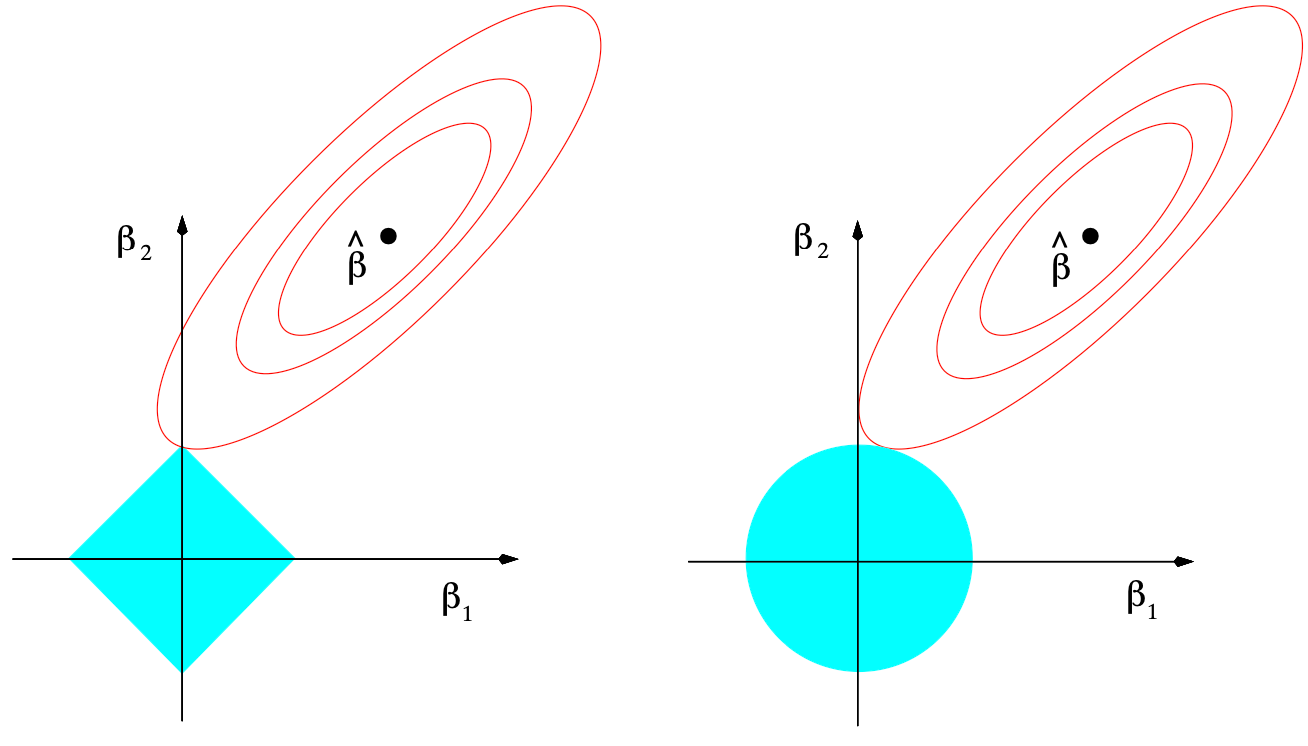
\includegraphics[scale=0.23]{figures/Estimation_picture.png}
    \end{center}
    \begin{itemize}
        \item \textbf{Ridge:} Penalty regions are circular (\(\ell_2\)-norm). Coefficients shrink uniformly.
        \item \textbf{Lasso:} Penalty regions are diamond-shaped (\(\ell_1\)-norm). Corners can force coefficients to zero.
        \item \textbf{Source:} Hastie, Tibshirani, \& Friedman (2009).
    \end{itemize}
\end{frame}

\begin{frame}
    \frametitle{Elastic Net Regression}
    \begin{itemize}
        \item \textbf{Definition:} Combines both \(\ell_1\) and \(\ell_2\) penalties.
        \[
            J^{\text{elastic net}}(\boldsymbol{\beta}) 
            = \frac{1}{2n}\sum_i\bigl(y_i - \beta_0 - \sum_j\beta_j x_{ij}\bigr)^2 
            + \lambda_e \Bigl((1-\alpha)\sum_j \beta_j^2 + \alpha \sum_j|\beta_j|\Bigr).
        \]
        \item \(\alpha \in [0,1]\) controls the \textbf{mix} between \(\ell_2\)-like and \(\ell_1\)-like behavior.
        \item \textbf{Why Elastic Net?}
        \begin{itemize}
            \item Balances the strengths of ridge (stability) and lasso (sparsity).
            \item Can outperform pure ridge/lasso in cases with correlated features.
        \end{itemize}
    \end{itemize}
\end{frame}

\begin{frame}
    \frametitle{Comparing Ridge, Lasso, and Elastic Net}
    \begin{columns}
    \column{.5\textwidth}
        \textbf{Ridge (\(\ell_2\))}: 
        \begin{itemize}
            \item Coefficients get \textit{shrunk} but \emph{not} set to zero.
            \item Good when all features have small contributions.
            \item Helps reduce variance from correlated predictors.
        \end{itemize}
        
        \textbf{Lasso (\(\ell_1\))}:
        \begin{itemize}
            \item Can set some coefficients to \textbf{zero} (\textit{feature selection}).
            \item More useful when many features may be truly irrelevant.
            \item Can struggle when predictors are highly correlated (tends to pick one).
        \end{itemize}
    \column{.5\textwidth}
        \textbf{Elastic Net}:
        \begin{itemize}
            \item A convex combination of \(\ell_1\) and \(\ell_2\) penalties.
            \item Offers some sparsity plus stability.
            \item Tuning involves \(\lambda\) \emph{and} \(\alpha\).
        \end{itemize}
        \vspace{0.5em}
        \textbf{Key Takeaway}: 
        \begin{itemize}
            \item Choose based on data structure and desired features.
            \item Use cross-validation to find optimal regularization parameters.
        \end{itemize}
    \end{columns}
\end{frame}

\begin{frame}
    \frametitle{Choosing the Regularization Parameter \(\lambda\)}
    \begin{itemize}
        \item \(\lambda\) (or \(\lambda_r\), \(\lambda_\ell\), etc.) controls the penalty strength:
        \begin{itemize}
            \item \(\lambda = 0 \rightarrow\) reverts to ordinary least squares (no penalty).
            \item \(\lambda \rightarrow \infty \rightarrow\) shrinks all coefficients toward 0.
        \end{itemize}
        \item \textbf{Cross-Validation:} 
        \begin{itemize}
            \item Systematically vary \(\lambda\) over a grid of values.
            \item Evaluate prediction error (MSE, MAE, etc.) on the validation set.
            \item Pick \(\lambda\) that minimizes validation error or has the best trade-off (e.g., 1-SE rule).
        \end{itemize}
        \item \textbf{Practical Tips:}
        \begin{itemize}
            \item Standardize features before applying regularization to ensure fair coefficient shrinkage.
            \item Watch for high correlation among features (especially for Lasso).
        \end{itemize}
    \end{itemize}
\end{frame}

\begin{frame}[fragile]
    \frametitle{Implementation and Practical Tips}
    \begin{itemize}
        \item \textbf{Scikit-learn Implementations:}
            \begin{itemize}
                \item \texttt{Ridge()} for ridge regression.
                \item \texttt{Lasso()} for lasso regression.
                \item \texttt{ElasticNet()} for elastic net.
            \end{itemize}
        \item \textbf{Example (Ridge):}
\begin{verbatim}
from sklearn.linear_model import Ridge
ridge_reg = Ridge(alpha=1.0)
ridge_reg.fit(X_train, y_train)
y_pred = ridge_reg.predict(X_test)
\end{verbatim}
        \item \textbf{Hyperparameter Tuning:}
            \begin{itemize}
                \item Use \texttt{GridSearchCV} or \texttt{RandomizedSearchCV} to find the best \(\alpha\).
                \item For ElasticNet, tune both \(\alpha\) (mixing ratio) and \(\lambda\).
            \end{itemize}
        \item \textbf{Common Pitfalls:}
            \begin{itemize}
                \item Forgetting to scale data can bias penalty terms.
                \item Over-penalizing: too high \(\lambda\) can underfit.
            \end{itemize}
    \end{itemize}
\end{frame}


\end{document}